

We define five hidden predicates for the three stages of the task. Figure \ref{fig:achitecture} illustrates these predicates and the stage they belong to. 
For predicate identification, we use the predicate \emph{isPredicate}. \emph{isPredicate(p)} indicates that the word in the position $p$ is an SRL predicate.

For argument identification and classification, we use the predicates \emph{isArgument}, \emph{hasRole} and \emph{role}. The atom \emph{isArgument(a)} signals that the word in the position $a$ is a SRL argument of some (unspecified) SRL predicate while \emph{hasRole(p,a)} indicates that the token at position $a$ is an argument of the predicate in position $p$. The predicate \emph{role(p,a,r)} corresponds to the decision that the argument in the position $a$ has the role $r$ with respect to the predicate in the position $p$.

Finally, for sense disambiguation we  define the predicate \emph{sense(p,e)} which signals that predicate in position $p$ has the sense $e$. 

\begin{figure}
\begin{center}
    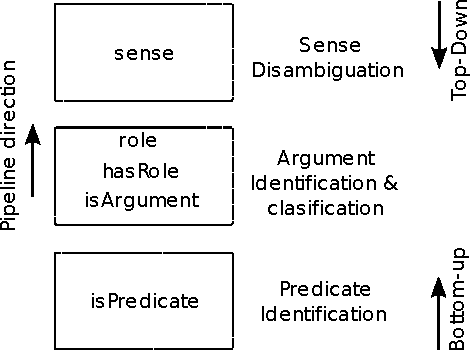
\includegraphics[scale=.70]{TaskArchitecture}
\end{center}
\caption{MLN hidden predicates divided in stages}
\label{fig:achitecture}
\end{figure}

\section{Local formulae}

A formula is local if its groundings relate any number of observed ground atoms to exactly one hidden ground atom. For example, a grounding of the local formula 
\[lemma(p,+l_1) \wedge lemma(a,+l_2) \Rightarrow hasRole(p,a)\]
can be seen in the Markov Network of Figure \ref{fig:local2}. It connects a hidden \emph{hasRole} ground atom to two observed \emph{lemma} ground atoms. Note that the ``+'' prefix for variables indicates that there is a different weight for each possible pair of lemmas $(l_1,l_2)$.

\begin{figure}
\begin{center}
    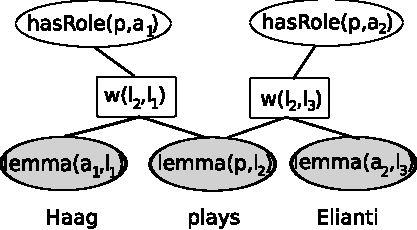
\includegraphics[scale=.70]{LocalFormula2}
\end{center}
\caption{Factor graph for the local formula in section \ref{sec:local}.}
\label{fig:local2}
\end{figure}

For the predicates \emph{isPredicate} and \emph{isArgument} we define the
following formuale:
\begin{description}
    \item[$Word$] a rule for the orthography of possible Predicate or Argument.
    \item[$Lemma_{-2,-1,1,2}$] for each lemma in a window of two previous and two following token a rule of possible Predicate or Argument.
    \item[$POSs_{-2,-1,1,2}$] for each POS in a window of two previous and two following tokens a rule of possible Predicate or Argument.
    \item[$CoarsePOS$] a rule for the previous and the following coarse POS tags of possible Predicate or Argument.
    \item[$CoarsePOS_2$] a rule for the two previous and two following corar POS tags of possible Predicate or Argument.
    \item[$DependecyChildren$] a rule for the dependencies of each child of possible Predicate or Argument.
    \item[$DependecyParent$] a rule for the dependencies of parent of possible Predicate or Argument.
    \item[$DependecyChildrenPOS$] a rule for the POS tag for each child  of possible Predicate or Argument.
    \item[$DependecyChildrenParPOS$] a rule for the POS tag of parent and each child  of possible Predicate or Argument.
    \item[$MFrame$] a rule for the MFrame of possible Predicate or Argument.
\end{description}



For the \emph{hasRole} and \emph{role} predicates we defined local formulae that aimed to reproduce the standard features used in previous work~\citep{xue04calibrating}. This also required us to develop dependency-based versions of the constituent-based features such as the syntactic path between predicate and argument, as proposed by \cite{xue04calibrating}. 

The remaining hidden predicates, \emph{isPredicate}, \emph{isArgument} and \emph{sense}, have local formulae that relate their ground atoms to properties of a contextual window around the token the atom corresponds to. For this we used the information provided in the closed track training corpus of the shared task (i.e. both versions of lemma and POS tags plus a coarse version of the POS tags). 




%Instead of describing the local feature set in more detail we refer the reader to our MLN model files.\footnote{\url{http://thebeast.googlecode.com/svn/mlns/conll08}} They can be used both as a reference and as input to our Markov Logic Engine\footnote{\url{http://thebeast.googlecode.com}}, and thus allow the reader to easily reproduce our results. We believe that this is another advantage of explicitly separating model and algorithms by using first order probabilistic logic languages.

\section{Global formulae}

\emph{Global} formulae relate several hidden ground atoms. We use them for two purposes: to ensure consistency between the decisions of all SRL stages and to capture some of our intuition about the task. We will refer to formulae that serve the first purpose as \emph{structural constraints}. 

% They aim to capture the relations between the hidden predicates, and ultimately of the stages of the SRL task. There are two types of global formulae: \emph{hard formulae} and \emph{soft formulae}. The hard formulae imposes constraints on the structure of the predicates. We can use hard formulae to solve the problem of coupling predicates.
For example, a structural constraint is given by the (deterministic) formula
\[role(p,a,r) \Rightarrow hasRole(p,a)\]
which ensures that, whenever the argument $a$ is given a label $r$ with respect to the predicate $p$, this argument must be an argument of $a$ as denoted by \emph{hasRole(p,a)}. Note that this formula by itself models the traditional ``bottom-up'' argument identification and classification pipeline: it is possible to not assign a role $r$ to an predicate-argument pair $(p,a)$ proposed by the identification stage; however, it is impossible to assign a role $r$ to token pairs $(p,a)$ that have not been proposed as potential arguments.

One example of another class of structural constraints is 
\[
hasRole(p,a)\Rightarrow\exists r.role(p,a,r)
\]
which, by itself, models an inverted or ``top-down'' pipeline. In this architecture the argument classification stage can assign roles to tokens that have not been proposed by the argument identification stage. However, it must assign a label to any token pair the previous stage proposes. 
%IV
Figure \ref{fig:global2} illustrates the structural formulae we use in form of a Markov Network.

The formulae we use to ensure consistency between the remaining hidden predicates are omitted for brevity as they are very similar to the bottom-up and top-down formulae we presented above.

For the SRL predicates that perform a labelling task (\emph{role} and \emph{sense}) we also need a structural constraint which ensures that not more than one label is assigned. For instance,
\[
(role(p,a,r_1) \wedge r_1 \neq r_2 \Rightarrow \neg role(p,a,r_2)  )
\]
forbids two different semantic roles for a pair of words. 

% thatrequires that for each \emph{hasRole} predicate there must be a SRL predicate in the postions $p$. This formula help us to relate two of the hidden predicates. The efect of the formula is similar to the bottom-up strategy where after identifing the the arguments of these are classified.

The global formulae that capture our intuition about the task itself can be further divided into two classes. The first one uses deterministic or \emph{hard} constraints such as
\begin{eqnarray*}
 &role\left(p,a_{1},r\right)\wedge \neg mod\left(r\right)\wedge a_{1}\neq a_{2}  \Rightarrow\\
  & \neg role\left(p,a_{2},r\right)
\end{eqnarray*}
which forbids cases where distinct arguments of a predicate have the same role unless the role describes a modifier.
%In this case we constrain to one semantic role to the words identify as proper arguments by the Palmer's heuristics. % ??

The second class of global formulae is \emph{soft} or nondeterministic. For instance, the formula  
\begin{eqnarray*}
  & lemma(p,+l) \wedge ppos(a,+p)  \\
  & \wedge hasRole(p,a)  \Rightarrow sense(p,+f) 
\end{eqnarray*}
is a soft global formula. It captures the observation that the sense of a verb or noun depends on the type of its arguments. Here the type of an argument token is represented by its POS tag.

%the relation between the \emph{hasRole} and \emph{sense} hidden predicates, together with the lemma of the SRL predicate and the POS tag of the argument. Figure \ref{fig:global2} is a graphical model representing the grounded version of this formula. %This formula does not imposes a structural constrain, but rather the link between the sense of the SRL predicate and its arguments.
%Why would this help?

\begin{figure}
\begin{center}
   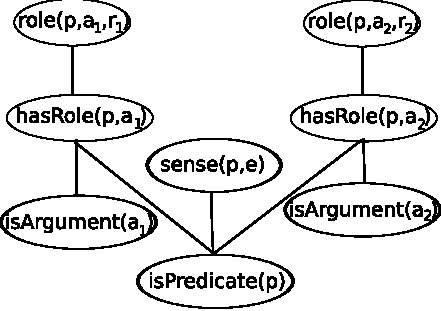
\includegraphics[scale=.70]{GlobalFormula2}
\end{center}
\caption{Markov Network that illustrates the structural constraints we use.}
\label{fig:global2}
\end{figure}






% Finally, to our last group of rules belongs the soft formulae and hard constrains with extra linguistic knowledge. Figure \ref{fig:global2} shows an example of soft formulae. An example, of hard constriain which uses extra linguistic knowledge is:
% \begin{eqnarray*}
%  & role\left(p,a_{1},r\right)\wedge arg\left(r\right)\wedge a_{1}\neq a_{2} & \Rightarrow\\
%   & \neg role\left(p,a_{2},r\right)
% \end{eqnarray*}
% In this case we constrain to one semantic role to the words identify as proper arguments by the Palmer's heuristics. % ??
%
%We have slit our global formulae into four groups. The first, are hard constrains which only involve one hidden predicate. The second one correspond to the hard constrains which involve more than one hidden predicate but follow a bottom-up strategy. This is conect two hidden predicates following the pipeline of the stages of the task. The top-down group group goes in a different direction. And finally, the fourth group contains the global formulae. In the section \ref{sec:results} we will explore how these relations contribute to the whole model. Table \ref{tbl:global} enumerate the global formulae used in this work.
%\begin{table}
%\begin{tabular}{|l|p{6cm}|}\hline
%Group & Description \\\hline
%1st   & There is one or less $role$ predicates for a pair of words (see Figure \ref{fig:hard1}.)\\
%      & There is one or less $frameLabel$ predicates for a word\\
%      & There are more than one $haslabel$ predicate for each word which is a possible argument by the Palmer heuristics\\\hline
%2nd   & If there is a $isPredicate(p)$ predicate, there must be a $frameLabel(p,_)$ predicate\\
%      & If thrre is a $isPredicate(p)$ predicate, there must be a $hasLabel(p,_)$ predicate\\      
%      & If there is a $hasLabel(p,a,_)$ predicate, there must be a $role(p,a,_)$ predicate\\\hline
%3rd   & If there is a $role(p,a,_)$ predicate, there must be a $hasLabel(p,a)$ predicate. \\
%      & If there is a $frameLabel(p,_)$ predicate, there must be a $isPredicate(p)$ predicate\\
%      & If there is a $hasLabel(p,_)$ predicate, there must be a $isPredicate(p)$ predicate.\\
%      & If there is a $hasLabel(_,a)$ predicate, there must be a $isArgument(a)$ predicate.\\\hline
%4th   & There shouldn't be two $hasLabel$ predicate for the which have as a predicate the same word, and the two arguments are prepositional phrases.\\
%      & There shouldn't be two predicates which overlap\\
%      & A $frameLabel$ predicated depends of the POS tags of the arguments of the predicate (see Figure \ref{fig:global1}\\
%      & For each proper argument defined by the Palmer heuristics there should be at most one $role$ predicate for that argument\\\hline
%      \end{tabular}
%\caption{Global formulae }
%\label{tbl:global}
%\end{table}
%


